\beginsong{Es, es, es und es}[
    % wuw={Volkslied, 1952 (ergänzt und vertont von Felicitas Kuckuck, 1957)},
    % bo={118},
    % pfii={64},
    % gruen={221},
    % kssiv={80},
    % siru={73},
]

% \beginverse
% \endverse
% 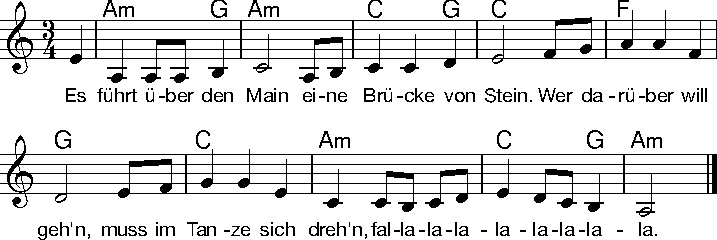
\includegraphics[draft=false, width=1\textwidth]{Noten/Lied035.pdf}
\transpose{-2}

\beginverse
\[G]Es, \[D]es, \[G]es und es, es \[Em]ist ein \[D]harter \[G]Schluß
\[G]Weil, \[D]weil, \[G]weil und weil, weil \[Em]ich aus \[D]Frankfurt \[G]muss!
Drum \[G]schlag ich Frankfurt \[D]aus dem Sinn und \[Em]wende mich Gott \[D]weiß \[A]wo\[D]hin. 
\[D7]Ich \[G]will mein \[D]Glück \[G]probieren, mar\[D7]schie\[G]ren,
\endverse

\beginverse
^Er, ^er, ^er und er, Herr ^Meister, ^leb er ^wohl!
^Er, ^er, ^er und er, Herr ^Meister, ^leb er ^wohl!
Ich ^sag's ihm grad frei ^in's Gesicht, seine ^Arbeit, die ^gefällt ^mir ^nicht!
^Ich ^will mein ^Glück pro^bieren, mar^schie^ren.
\endverse

\beginverse
^Sie, ^sie, ^sie und sie, Frau ^Meist'rin ^leb sie ^wohl!
^Sie, ^sie, ^sie und sie, Frau ^Meist'rin ^leb sie ^wohl!
Ich ^sag's ihr grad frei ^in's Gesicht, Ihr ^Speck und Kraut, der ^schmeckt ^mir ^nicht!
^Ich ^will mein ^Glück pro^bieren, mar^schie^ren.
\endverse

\beginverse
^Sie, ^sie, ^sie und sie, Jungfer ^Köchin, ^leb sie ^wohl!
^Sie, ^sie, ^sie und sie, Jungfer ^Köchin, ^leb sie ^wohl!
Hätt' ^sie das Essen besser ^angericht' so ^wär ich auch ge^wan^dert ^nicht!
^Ich ^will mein ^Glück pro^bieren, mar^schie^ren.
\endverse

\beginverse
^Er, ^er, ^er und er, Herr ^Wirt, nun ^leb' er ^wohl!
^Er, ^er, ^er und er, Herr ^Wirt, nun ^leb' er ^wohl!
Hätt ^er die Kreid' nicht ^doppelt geschrieben, Wär' ^ich noch länger ^da^ge^blieben!
^Ich ^will mein ^Glück pro^bieren, mar^schie^ren.
\endverse

\beginverse
^Ihr, ^ihr, ^ihr und ihr, ihr ^Jungfern ^lebet ^wohl!
^Ihr, ^ihr, ^ihr und ihr, ihr ^Jungfern ^lebet ^wohl!
Ich ^wünsche euch zu ^guter Letzt, einen ^ander'n, der mein' ^Stell' ^er^setzt!
^Ich ^will mein ^Glück pro^bieren, mar^schie^ren.
\endverse

\beginverse
^Ihr, ^ihr, ^ihr und ihr, ihr ^Brüder ^lebet ^wohl!
^Ihr, ^ihr, ^ihr und ihr, ihr ^Brüder ^lebet ^wohl!
Hab ^ich euch was zu^leid getan, So ^bitt' ich um Ver^zeih^ung ^an!
^Ich ^will mein ^Glück pro^bieren, mar^schie^ren.
\endverse

\endsong
